%!TEX program = xelatex
\documentclass[12pt]{article}
% --importing files packages
\usepackage[subpreambles=true]{standalone}
\usepackage{pdfpages}
\usepackage{import}
\usepackage{customstyle}
\usepackage{graphicx}
\usepackage[space]{grffile}
\usepackage{makecell}

\begin{document}
% did not work, not sure why
%\import{pages/}{titlePage.tex}

%% ---
\inputencoding{utf8} 
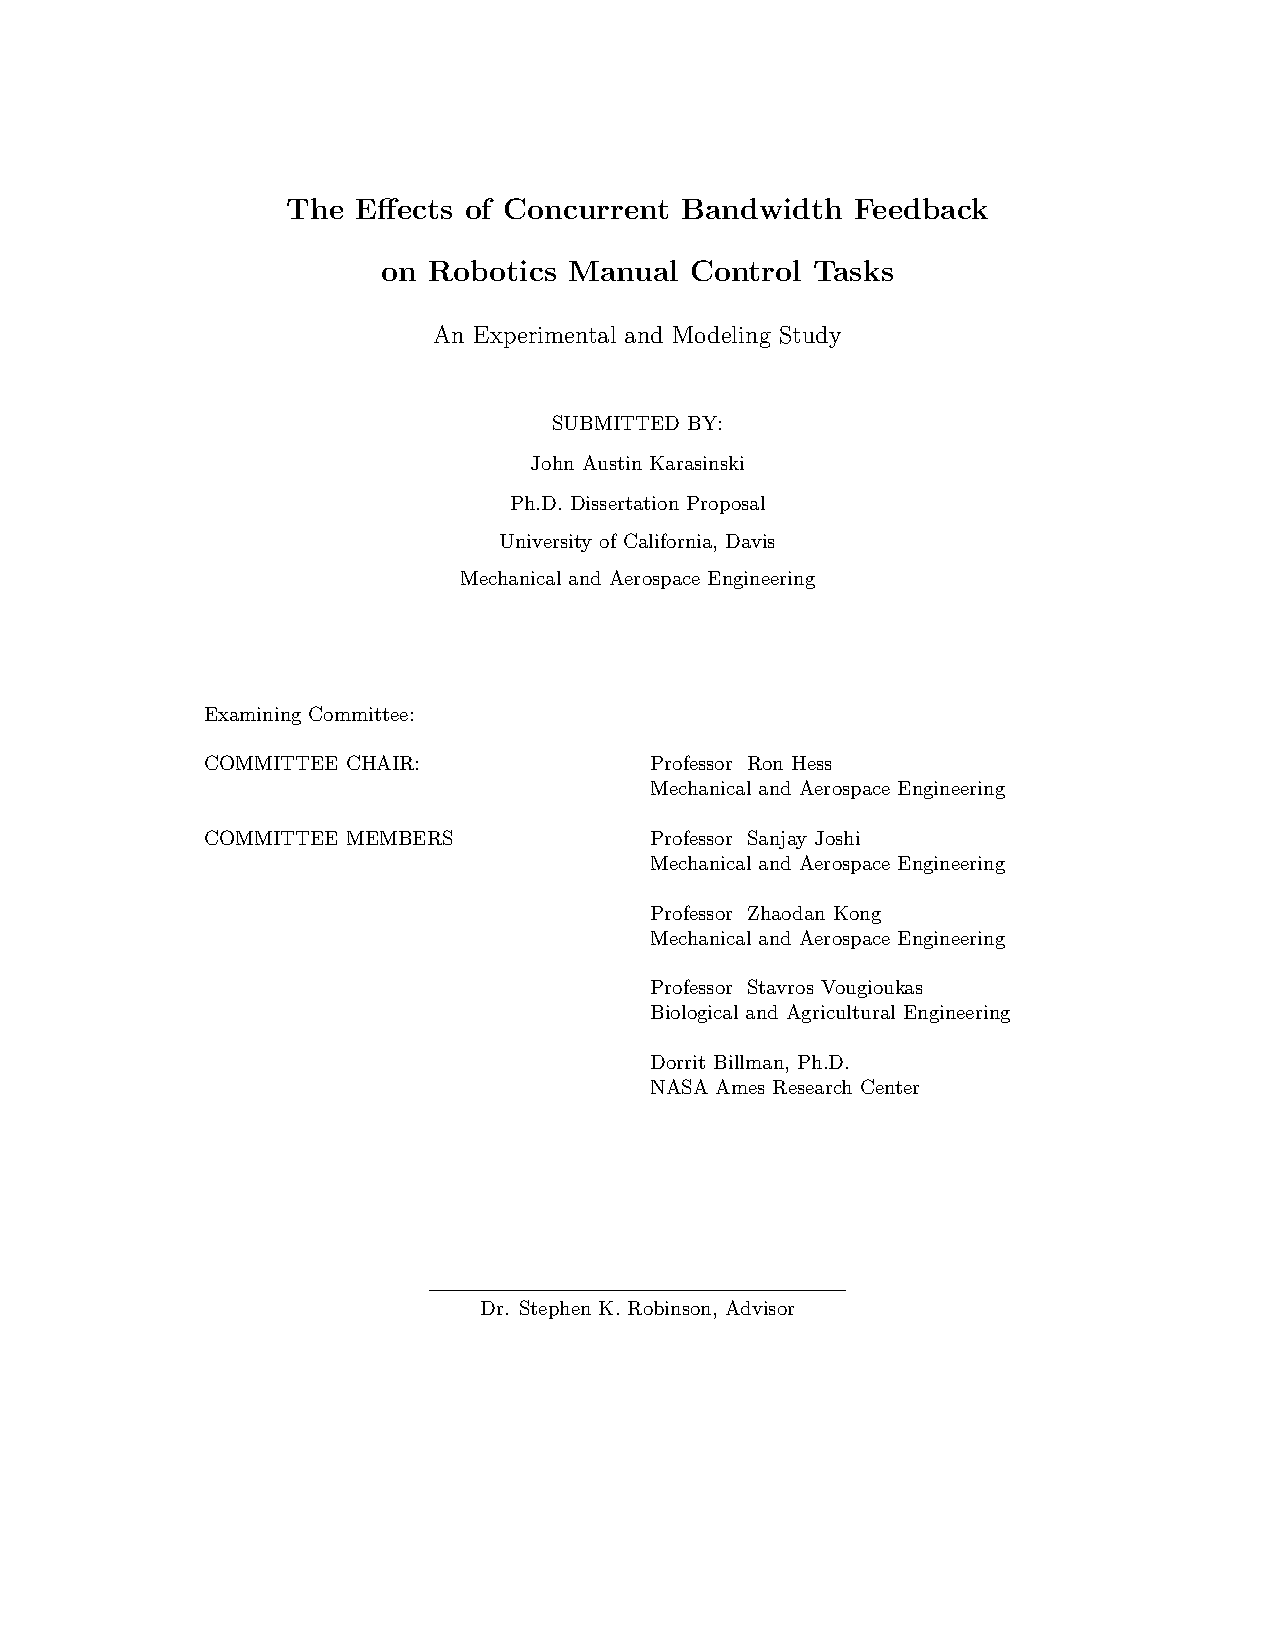
\includepdf{./pages/titlePage}
% \includepdf{./pages/coverPageSigned}
\newpage \pagenumbering{roman}
\tableofcontents 
\newpage \pagenumbering{arabic} \setcounter{page}{1}
\import{pages/}{problem}
% \newpage
\import{pages/}{background}
% \newpage
\import{pages/}{strategy}
% \newpage
\import{pages/}{results}
% \newpage
\import{pages/}{conclusions}

\newpage
\bibliographystyle{nar}
{\sffamily \footnotesize \setstretch{.5}
\bibliography{bib}
}
\end{document}
